\documentclass[10pt]{beamer}

\usetheme[progressbar=frametitle]{metropolis}

\usepackage{booktabs}
\usepackage[scale=2]{ccicons}

\usepackage{pgfplots}
\usepgfplotslibrary{dateplot}

\usepackage{xspace}
\newcommand{\themename}{\textbf{\textsc{Rendezvous}}\xspace}

\title{Rendezvous Search for Power Save Design}
\subtitle{for wifi infrastructure mode}
\date{\today}
\author{Yang Hang}
\institute{Gratitude Institute of Communication Engineering }
\titlegraphic{\hfill
\includegraphics[height=1.5cm]{logo}}

\begin{document}

\maketitle

\begin{frame}{Table of contents}
    \setbeamertemplate{section in toc}[sections numbered]
    \tableofcontents[hideallsubsections]
\end{frame}

\section{Rendezvous Search}
\begin{frame}{\themename Search Problem}
    Two people who are placed \textbf{randomly} in a known \textbf{search region} and move about at unit speed to find each other in the least expected time. This time is called the \themename  Value of the \textbf{region}.  

    \alert{Problem (Astronaut Problem)} \textit{Two astronauts land on a spherical body that is much larger than the detection radius(which they can see each other). The body does not have a fixed orientation in space, nor does it have an axis of rotation so that they cannot have common notion of position or direction. Given unit walking speeds for both astronauts, how should they move about so as to minimize the expected meeting time T?}\cite{alpern1995rendezvous}
\end{frame}

\begin{frame}{Rendezvous Search Model}
    $Q$: the region the two players will be located. \\
    $R(Q)$: the rendezvous value the region. \\
    $\mathbb{S}_i $: strategy set of player $i, i = 1,2$. \\
    $T$: the least meeting time. 
    \begin{equation}
        \label{ss} % strategy space
        \mathbb{S}_i = \lbrace s: [0, \infty)\rightarrow Q, d(s(t), s(t^\prime)) \leq |t-t^\prime| \rbrace
        \end{equation}
        \begin{equation}
            \label{lmt} % least meeting time
            T = T(s_1,s_2) = \inf \lbrace t: d(s_1(t), s_2(t)) \leq r \rbrace 
        \end{equation}
        \begin{equation}
            \label{rv} % rendezvous value
            R(Q) = \min_{s_1 \in \mathbb{S}_1, s_2 \in \mathbb{S}_2} {T(s_1, s_2)}
        \end{equation}
        $d(g,h)$: distance between $g$ and $h$.\\
        $x_0$: initial location.\\
        $r$ is the detection range. 
    \end{frame}
    \section{Power Save of WiFi MAC}
    \begin{frame}{Power Save of infrastructure WiFi}
        In infrastructure mode, we only care the energy consumption of STA. And because STAs could send the up-link(UL) packets immediately once the UL packet arriving, we regard UL as efficient transmission. 
        We care DL transmission.

        A legacy power save mode(PSM) is illustrated here, with parameter beacon interval($BI$) and listen interval($LI$). See next slide. 
    \end{frame}
    \begin{frame}{PSM}
        \begin{figure}
            \centering
            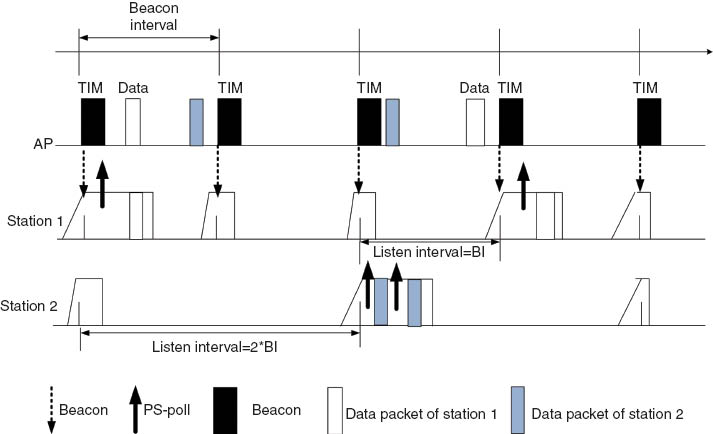
\includegraphics[scale=0.8]{./figure/legacy_PSM.jpg}
            \caption{Illustration of PSM \cite{xie2014adaptive}}
            \label{PSM}
        \end{figure}
    \end{frame}
    \section{Rendezvous search for PS on WiFi}
    \begin{frame}{Intuition of PS on WiFi}
        Since in WiFi, if no PS, STAs will stay \textbf{active} all the time, \textbf{sending}, \textbf{receiving} packets, or \textbf{idle}(ready for transmission). All the three modes above are high power-consumed. Another mode -- \textbf{sleep mode} which disables sending and receiving but consume lower power.

        It is intuitive that working in idle mode is kind of waste of energy. That's indeed what PS is doing -- a mechanism reduce duration of idle mode by implementing sleep mode to save energy. The constraint are \textbf{packet access delay} and \textbf{success rate of transmission}. 
    \end{frame}

    \begin{frame}{Rendezvous for PS on WiFi}
        We consider the \textbf{P2P} first. CSMA/CA is ignored here. 
        Only \textbf{DL} is what we care, no UL. And given DL traffic pattern $\lbrace N(t), t\geq 0 \rbrace$.  

        Imagine the \textbf{search region} as timeline here, a directed line. 
        $STA$ as player $I$, AP as player $II$. Recall the equation \ref{ss},\ref{lmt},\ref{rv}, then the model for PS on wifi would be like:
        \begin{equation}
            \label{PS_ss}
            \mathbb{S}_i = \lbrace s:\mathbb{R}^+\rightarrow \mathbb{R}^+ \rbrace
        \end{equation}
        \begin{equation}
            \label{PS_lmt}
            T = \inf\lbrace s_1(t): s_1(t) = s_2(t), N(s_1(t)) \geq 1 \rbrace
        \end{equation}
        $\mathbb{S}_i $: strategy set of player $i = 1,2$. \\
        $T$: the least meeting time(MT), here means the time of \textbf{successful transmission}. 
    \end{frame}

    \begin{frame}{Rendezvous for PS on WiFi}
        $T_d$: Packet access delay. \\
        $T_{a_1}$: The arrival time of first DL packet.  
        \begin{equation}
            T_d = T - T_{a_1} 
        \end{equation}
        As for energy consumption of STA, power-consumption is based on the working mode: 
        \begin{equation}
            \label{PowerConsumption}
            P_1(t) =
            \begin{cases}
                P_0, if\ s_1(t)\neq t, sleep\\
                P_1, if\ s_1(t) = t\, \& \, N(t) = 0, idle
            \end{cases}
        \end{equation}
        \begin{figure}[h!]
            \centering
            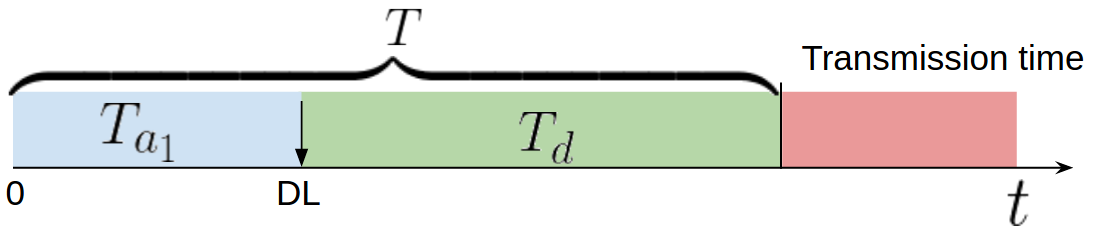
\includegraphics[scale=0.25]{./figure/RS_timeline.png}
            \caption{Explanation on timeline}
            \label{Timeline}
        \end{figure}
    \end{frame}

    \begin{frame}{Rendezvous for PS on WiFi}
        For receiving mode, we assume it a constant and because it is essential for transmission, we don't care it. We name a \textbf{cost energy} which is used for preparation for packet reception. 
        Then the \textbf{cost energy} is as following:
        \begin{equation}
            \label{CostEnergy}
            E = \int_0^T P_1(t)\,\mathrm{d}t % integral format
        \end{equation} 
        We have the optimization formula as follows:
        \begin{equation}
            \label{OptimizationFormula}
            \begin{split}
                \min\ & E \\
                \textrm{s.t.} & T_d \leq \tau
            \end{split}
        \end{equation}
        $\tau$: maximum tolerated packet access delay. 
    \end{frame}

    \begin{frame}{Rendezvous Search model for PSM}
        Recall the PSM, we can see it as a strategy for player $I$ and player $II$, i.e. STA and AP. Then the we have: 
        \begin{equation}
            \label{ConcreteStrategy}
            \begin{split}
                s_1(t) &= kLI, if \, (k-1)LI < t \leq kLI \\
                s_2(t) &= kBI, if \, (k-1)BI < t \leq kBI, k = 1,2...
            \end{split}
        \end{equation}
        $LI$: listen interval. \\
        $BI$: beacon interval. \\
        We plot the two strategy "paths", given $BI = 100, LI = 2BI$. See next slide. 
    \end{frame}

    \begin{frame} % figure of 
        \begin{figure}
            \centering
            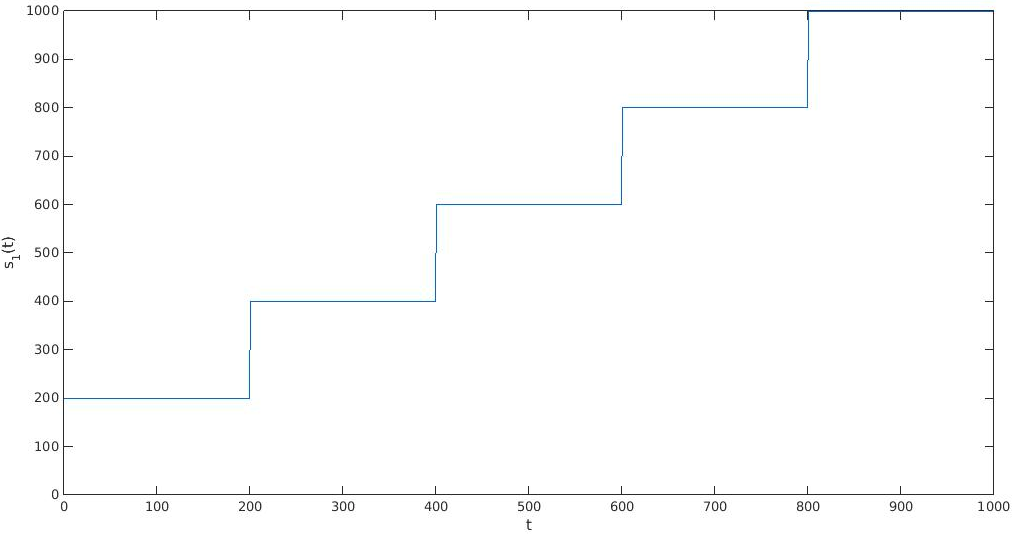
\includegraphics[scale=0.23]{./figure/s1_sta_plot.png}
            %\caption{Domain of $f$}
            \label{s1}
        \end{figure}%
        \begin{figure}
            \centering
            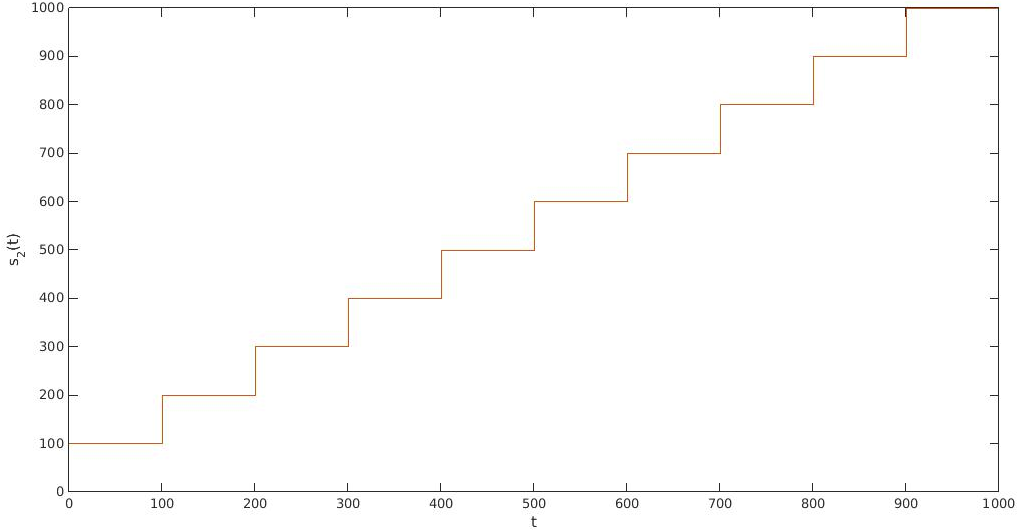
\includegraphics[scale=0.23]{./figure/s2_ap_plot.png}
            %\caption{n=5}
            \label{s2}
        \end{figure}
    \end{frame}
    \section{Issues}
    \begin{frame}{Issues}
        Rendezvous Search(RS) is a brand new prospective way to see PS of WLAN. It is more general prospective. Many existing PSMs can be modeled as strategies into the RS framework. However, many confuses exist here.   
        \begin{enumerate}
            \item RS is a model of two players or multiple players meeting together. For multiple players in WLAN, it needs modification. 
            \item RS cares the first meeting time(MT); that's why we focus on the transmission of \text{first} DL packet.   
            \item RS cares expected value of MT; but in WLAN, we need some QoS(worst case matters).   
            \item Validation, the model simplifies so much that we need to think of some way to validate.
            \item Continuous \textbf{vs} Discrete time. 
        \end{enumerate}
    \end{frame}
    \begin{frame}{Issues}
        We will do: 
        \begin{enumerate}
            \item Calculate a theoritical optimal energy-consumption of such a "region" given a arrival pattern.
            \item Propose an optimal strategy(algorithm). 
        \end{enumerate}
    \end{frame}

    \plain{Thanks}

    \begin{frame}[allowframebreaks]{References}
        \bibliography{demo}
        \bibliographystyle{abbrv}
    \end{frame}

    \end{document}
